\clearpage\section{Chapter 9: Classes and Objects}
Classes are user-defined data types that model the information and
behavior of elements in the application domain. \ In Unicon they are
records with associated procedures, called methods. Instances of these
special record types are called objects. In this chapter you will learn
how to:

\begin{itemize}
\item Draw diagrams that show class names, attributes, and methods
\item Write corresponding code for classes and their methods
\item Create instances of classes and invoke methods on those objects
\end{itemize}
\subsection{Class Diagrams}
Modeling a software system begins with the task of identifying things
that are in the system and specifying how they are related. A class
diagram shows a static view of relationships between the main kinds of
elements that occur in the problem domain. A class diagram is a
data-centric, object-centric model of the program. In contrast, a
user-centric view is provided by use cases. \index{class!diagrams}Class
diagrams have several basic components.

Classes are represented by rectangles. A
{\textquotedbl}class{\textquotedbl} denotes a concept of the
application domain that has state information (depicted by named
\index{attribute!class}\textit{attributes}) and/or behavior (depicted
by named \index{operations}operations, or \textit{methods}) significant
enough to be reflected in the model. Inside the rectangle, lines
separate the class name and areas for attributes and operations. Figure
9-1 shows an example class.

\bigskip

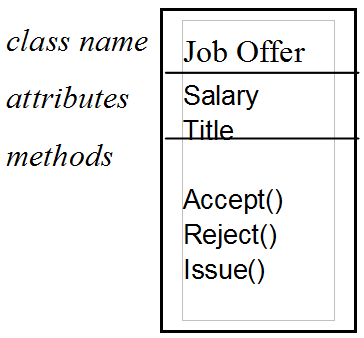
\includegraphics[width=2.5in,height=2.1335in]{ub-img/umlclass.png} 

{\sffamily\bfseries Figure 9-1:}
{\sffamily Class Job Offer has two Attributes and Three Methods}

\bigskip

When an object model is implemented, classes in the model are
implemented using programming language classes, which are described in
the next section. The degree of separation between the notion of a
class in the model and in the implementation depends on the programming
language. In the case of Unicon, the separation is minimal, because
built-in types such as lists and tables take care of almost all data
structures other than those introduced specifically to model
application domain elements. In the case of C++ or \index{Java}Java,
many additional implementation artifacts typically have to be
represented by classes.

The same class can appear in many class diagrams to capture all of its
relationships with other classes. Different diagrams may show different
levels of detail, or different aspects (projections) of the class
relevant to the portion of the model that they depict. In the course of
modeling it is normal to start with few details and add them gradually
through several iterations of the development process. Several kinds of
details may be added within a class. Such details include:

\begin{itemize}
\item The \index{visibility!within class}\textit{visibility} of
attributes and operations. A plus sign (+) before the attribute name
indicates that the attribute is \index{public}public and may be
\index{reference}referenced in code external to the class. A minus sign
(-) before the attribute name indicates that the attribute is
\index{private}private and may not be referenced in code outside the
class.
\item Types, initial values, and properties of attributes
\item Static properties of the class that will not be relevant at
run-time
\end{itemize}
Attribute names may be suffixed with a colon and a type, an equal sign
and a value, and a set of properties in curly braces. Figure 9-2 shows
two very different levels of detail for the same class. Each level of
detail is appropriate in different contexts.

\bigskip

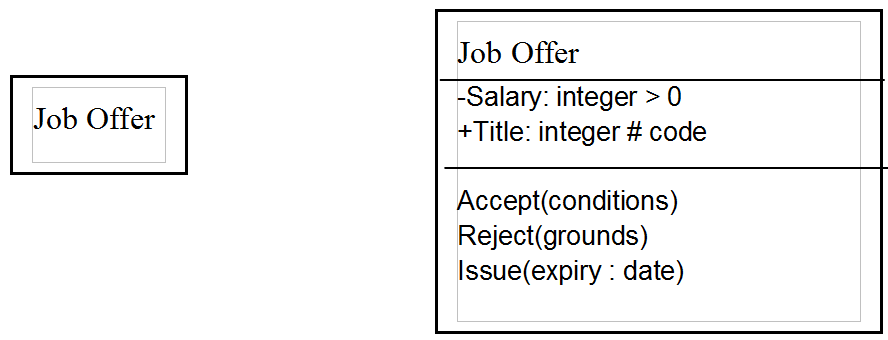
\includegraphics[width=4in,height=2.2in]{ub-img/lodetail.png} 

{\sffamily\bfseries Figure 9-2:}
{\sffamily A Class is Drawn with Different Levels of Detail in
 Different Diagrams}

\bigskip

You can draw rectangles with names of classes inside them all day, but
unless they say something about program organization, such diagrams
serve little purpose. The main point of drawing a class diagram is not
the classes; it is the relationships between classes that are required
by the model. These relationships are called
\index{association}\textit{associations}. In a class diagram,
associations are lines that connect classes. Accompanying annotations
in the diagram convey relevant model information about the
relationships. The details of associations and their implementation are
described in chapter 10.

\subsection[Declaring Classes]{Declaring Classes}
\index{class!declaration}In Unicon program code, the syntax of a class
is: 

\iconcode{
class foo(attribute1, attribute2, attribute3, ...) \\
\>   \# procedures (methods) to access class foo objects \\
\ \\
\# code to initialize class foo objects \\
end
}

The procedures that manipulate class objects are called
\index{method}\textit{methods}. Methods define a
class{\textquotesingle} interface with the rest of the program. The
syntax of a method is that of a procedure: 

\iconcode{
method bar(param1, param2, param3, ...) \\
\>   \# Unicon code that may access fields of a class foo object \\
end
}

Execution of a class method is always associated with a given object of
that class. The method has access to an implicit
\index{variable!implicit}\index{variable}variable called
\index{self}\textsf{self} that is a record containing fields whose
names are the attributes given in the class declaration. Fields from
the \textsf{self} variable are directly accessible by name. In addition
to methods, classes may also contain regular procedure, global, and
record declarations; such declarations have the standard semantics and
exist in the global name space. 

\subsection{Object Instances}
Like records, \index{instances!class object}instances of a class type
are created with a \index{constructor!class}constructor function whose
name is that of the class. Instances of a class are called objects, and
behave similar to records. The fields of an instance generally
correspond directly to the class attributes. Fields may be initialized
explicitly in the constructor in exactly the same way as for records.
For example, after defining a \textsf{class foo(x, y)} one may write: 

\iconcode{
procedure main() \\
\>   f := foo(1, 2) \\
end
}

In this case \texttt{x} would have the value \textsf{1}, and \textsf{y}
would have the value \textsf{2}, as would be the case for a record
type. The fields of an object do not have to be initialized by a
parameter passed to the class constructor. Many constructors initialize
objects{\textquotesingle} fields to some standard value. In this case,
the class declaration includes an \index{initially}\textsf{initially}
section after its methods are defined and before its end. An
\textsf{initially} section is just a special method that is invoked
automatically by the system when it creates each instance of the class.

An \textsf{initially} section begins with the reserved word
\textsf{initially} and an optional parameter list, followed by lines of
code that are executed whenever an object of that class is constructed.
These lines typically assign values to the attributes of the object
being created.

For example, suppose you want an enhanced table type that permits
sequential access to elements in the order they are inserted into the
table. You can implement this using a combination of a list and a
table, both of which would be initialized to the appropriate empty
structure: 

\iconcode{
class taque(L, T) \# pronounced {\textquotedbl}taco{\textquotedbl} \\
\ \\
\>   \# methods to manipulate taques, \\
\>   \# e.g. insert, index, foreach... \\
\ \\
initially \\
\>   L := [ ] \\
\>   T := table() \\
end
}

\noindent
In such a case you can create objects without including arguments to the
class constructor: 

\iconcode{
procedure main() \\
\ \ \ mytaque := taque() \\
end
}

In the absence of an \textsf{initially} section, missing arguments to a
constructor default to the null value. Together with an
\textsf{initially} section, the class declaration looks like a
procedure that constructs objects of that class. Note that you may
write classes with some fields that are initialized explicitly by the
constructor while other fields are initialized automatically in the
\textsf{initially} section. In this case you should either declare the
automatically initialized fields after those that are initialized in
the constructor, or insert \textsf{\&null} in the positions of the
automatically initialized fields in the constructor. The parameters to
the constructor are exactly in the order they appear in the class
declaration.

This default semantics for constructor parameters is awkward in some
cases, so there is an alternative. \ The \textsf{initially} section is
really just a special method, and it is allowed to take a parameter
list just like any other method. When an initially section includes a
parameter list, no implicit initialization of objects{\textquotesingle}
fields is performed. This frees the constructor from having the same
number and order of parameters as the declared class fields. In the
following class, the third field is initialized from constructor
parameter \textsf{x}, overriding the default behavior of initializing
fields in the declared order. This capability becomes important in
large classes with many fields.

\iconcode{
class C(a, b, c) \\
initially(x) \\
\>   c := x \\
end
}

\subsection{Object Invocation}

Once you have created an object with a class constructor, you manipulate
the object by invoking methods defined by its class. Since objects are
both procedures and data, object \index{invocation!object
method}invocation is a combination of a procedure call and a record
access. The syntax is

\iconcode{
\>   object . methodname ( arguments )}

If an object{\textquotesingle}s class is known, object methods can also
be called using a normal procedure call. This allows object oriented
Unicon code to be called from Icon. Called as a procedure, the name of
a method is prefixed with the class name and an underscore character.
The object itself is always the first parameter passed to a method. In
the absence of inheritance (discussed in the next chapter) if
\textsf{x} is an object of class \textsf{C},
\textsf{x.method(arguments)} is equivalent to \textsf{C\_method(x,
arguments)}.

Although object methods can be called using procedure calls, the field
operator has the advantage that it handles inheritance and polymorphism
correctly, allowing algorithms to be coded generically using
polymorphic operations. Generic algorithms use any objects whose class
provides the set of methods used in the algorithm. Generic code is less
likely to require change when you later enhance the program, for
example adding new \index{subclass}subclasses that inherit from
existing ones. In addition, if class names are long, the field syntax
is considerably shorter than writing out the class name for the
invocation. Using the taque example: 

\iconcode{
procedure main()\\
\>   mytaque := taque() \\
\>   mytaque.insert({\textquotedbl}greetings{\textquotedbl},
{\textquotedbl}hello{\textquotedbl}) \\
\>   mytaque.insert(123) \\
\>   every write(mytaque.foreach()) \\
\>   if (mytaque.index({\textquotedbl}hello{\textquotedbl})) then \\
\>\>    write({\textquotedbl}, world{\textquotedbl}) \\
end
}

For object-oriented purists, using the field operator to invoke an
object{\textquotesingle}s methods in this manner is the only way to
access an object. In Unicon, visibility issues such as
{\textquotedbl}public{\textquotedbl} and
{\textquotedbl}private{\textquotedbl} are best addressed in an
application{\textquotesingle}s design and documentation stages. A good
starting point is to consider all fields
{\textquotedbl}private{\textquotedbl} and all methods
{\textquotedbl}public{\textquotedbl}. Nevertheless, an object is just a
kind of record, complete with record-style field access.

Direct external access to an object{\textquotesingle}s data fields using
the usual field operator is not good practice, since it violates the
principle of encapsulation. Within a class method, on the other hand,
access to an object{\textquotesingle}s attributes is expected. The
implicit object named \textsf{self} is used under the covers, but
attributes and methods are referenced by name, like other variables.
The taque insert method is thus: 

\iconcode{
method insert(x, key) \\
\>   /key := x \\
\>   put(L, x) \\
\>   T[key] := x \\
end
}

The \textsf{self} object allows field access just like a record, as well
as method invocation like any other object. Using the \textsf{self}
variable explicitly is rare.

\subsection{Comparing Records and Classes by Example}
The concepts of classes and objects are found in many programming
languages. The following example clarifies the object model adopted by
Unicon and provides an initial impression of these
concepts{\textquotesingle} utility in coding. To motivate the
constructs provided by Unicon, our example contrasts conventional Icon
code with object-oriented code that implements the same behavior.

\subsubsection{Before Objects}

Suppose you are writing some text-processing application such as a text
\index{editor}editor. Such applications need to be able to process
structures holding the contents of various text files. You might begin
with a simple structure like the following: 

\iconcode{
record buffer(filename, text, index)}

\noindent
where \textsf{filename} is a string, \textsf{text} is a list of strings
corresponding to lines in the file, and \textsf{index} is a marker for
the current line at which the buffer is being processed. Icon record
declarations are global; in principle, if the above declaration needs
to be changed, the entire program must be rechecked. A devotee of
structured programming would likely write procedures to read the buffer
in from a file; write it out to a file; examine, insert and delete
individual lines; and so on. These procedures, along with the record
declaration given above, can be placed in their own source file
(\textsf{buffer.icn}) and understood independently of the program(s) in
which they are used. Here is one such procedure: 

\iconcode{
\# read a buffer in from a file \\
procedure read\_buffer(b) \\
\>   f := open(b.filename) {\textbar} fail \\
\>   b.text := [ ] \\
\>   b.index := 1 \\
\>   every put(b.text, !f) \\
\>   close(f) \\
\>   return \\
end
}

There is nothing wrong with this example; in fact its similarity to the
object-oriented example that follows demonstrates that a good, modular
design is the primary effect encouraged by \index{object-oriented
programming}object-oriented programming. Using a separate source file
to contain a record type and those procedures that operate on the type
allows an Icon programmer to maintain a voluntary encapsulation of that
type. 

\subsubsection{After Objects}
Here is part of the same buffer abstraction coded in Unicon. This
example lays the groundwork for some more substantial techniques to
follow. Methods are like procedures that are always called in reference
to a particular object (a class instance).

\iconcode{
class buffer(filename, text, index) \\
\>   \# read a buffer in from a file \\
\>   method read() \\
\>   \ \ \ f := open(filename) {\textbar} fail \\
\>   \ \ \ text := [ ] \\
\>   \ \ \ index := 1 \\
\>   \ \ \ every put(text, !f) \\
\>   \ \ \ close(f) \\
\>   \ \ \ return \\
\>   end \\
\>   \# ...additional buffer operations, including method erase() \\
initially \\
\>   if {\textbackslash}filename then read() \\
end
}

This example does not illustrate the full object-oriented style, but it
is a start. The object-oriented version offers encapsulation and
polymorphism. A separate name space for each class{\textquotesingle}s
methods allows shorter names. The same method name, such as
\textsf{read()} in the \ example, can be used in each class that
implements a given operation. This notation is more concise than is
possible with procedures. More importantly it allows an algorithm to
work on objects of any class that implements the operations required by
that algorithm. 

Consider the initialization of a new buffer. Constructors allow the
initialization of fields to values other than \textsf{\&null}. In the
example, the \textsf{read()} method is invoked if a filename is
supplied when the object is created. This can be simulated using
records by calling a procedure after the record is created; the value
of the \index{constructor!record}constructor is that it is automatic.
The programmer is freed from the responsibility of remembering to call
this code everywhere objects are created in the client program(s). This
tighter coupling of \index{memory allocation}memory allocation and its
corresponding initialization removes one more source of program errors,
especially on multi-programmer projects. 

The observations in the preceding two paragraphs share a common theme:
the net effect is that each piece of data is made responsible for its
own behavior in the system. Although this example dealt with simple
line-oriented text files, the same methodology applies to more abstract
entities such as the components of a
\index{compiler}compiler{\textquotesingle}s grammar.

The example also illustrates an important scoping issue. Within class
buffer, method \textsf{read()} effectively makes the regular built-in
function \textsf{read()} inaccessible! You should be careful of such
conflicts. It would be easy enough to capitalize the method name to
eliminate the problem. If renaming the method is not an option, as a
last resort you could get a reference to the built-in function
\textsf{read()}, even within method \textsf{read()}, by calling
\textsf{proc({\textquotedbl}read{\textquotedbl}, 0)}. The function
\textsf{proc()} converts a string to a procedure; supplying a second
parameter of 0 tells it to skip scoping rules and look for a built-in
function by that name.

{\sffamily
Summary}

Classes are global declarations that define a record data type and the
set of procedures that operate on that type. Instances of a class type
are called objects, and are normally manipulated solely by calling
their associated methods. Within a class, an object{\textquotesingle}s
fields are accessed as variables without the usual record dot notation,
and an object{\textquotesingle}s methods may be invoked by name, with
an appearance similar to ordinary procedure calls.


\bigskip

\clearpage
\bigskip
